%Balíčky
\documentclass[a4paper,10pt,twoside]{article}
\usepackage[utf8]{inputenc} %kodovani, abychom mohli jednoduse psat diakriticka pismena
\usepackage[english]{babel}
\usepackage{pifont}
\usepackage{graphicx} %pro vkladani obrazku
\usepackage{color}
\usepackage{fancyhdr} %zahlavi a zapati
\usepackage{ifpdf}
\usepackage{amssymb}
\usepackage{booktabs}
\usepackage{subfigure}
\usepackage{titlesec}
\usepackage[multiple]{footmisc}
\usepackage{color}       % pro zvýraznění textu barvou
\usepackage{multirow} 
\usepackage{multicol}
\usepackage{amsmath}
\usepackage{sectsty}
\usepackage[justification=centering]{caption}
\usepackage[top=1.5cm, left=3cm, right=3cm, bottom=2cm, headheight=26pt, includeheadfoot]{geometry}
\usepackage[colorlinks=false,urlcolor=black]{hyperref}
\usepackage{xcolor}
\usepackage{listings}
\hypersetup{
    colorlinks=true,
    linkcolor=black,
    filecolor=black,      
    urlcolor=black,
    citecolor=black
}
\allsectionsfont{\rmfamily} 

\sectionfont{\huge}
\subsectionfont{\LARGE}
\subsubsectionfont{\Large}

\def\nazevprace{\Large{Creation of a new GRASS GIS startup mechanism}}
\def\nazevpraceEN{\large{Tvorba nového startovacího mechanismu v prostředí GRASS GIS}}

\begin{document}
\sloppy
\setlength{\parskip}{8pt}

%%  ÚVODNÍ STRÁNKA %%%%%%%%%%%%%%%%%%%%%%%%%%%%%%%%%%%%%%%%%%%%%%

\pagestyle{empty} % vypne číslování stránek na úvodní straně

\begin{center}

\LARGE
\textsc{Czech Technical University in Prague} \\
\textsc{Faculty of civil engineering} \\

\bigskip

\large
\textsc{Department of Geomatics} \\

\vspace{6ex}

\begin{figure}[hbt!] %vlozeni loga
\begin{center}

\includegraphics[width=5.5cm]{pictures/logo_cvut.png} 
\end{center}
\end{figure}

\vspace{20ex}

\LARGE{MASTER'S THESIS}\\
\bigskip
\bigskip
\textsc{\nazevprace} \\
\smallskip
\textsc{\nazevpraceEN} \\

\mbox{}
\vfill

\normalsize
\textsc{\author} \\
\bigskip
\normalsize
\textrm{Supervisor: Ing. Martin Landa Ph.D.} \\

\vspace{10ex}
\large
\textrm{2020 Prague} \hfill
\textrm{Bc. Linda KLADIVOVÁ} \\

\end{center}

%% 2. STRÁNKA ZŮSTANE PRÁZDNÁ

\newpage ~ \newpage
\thispagestyle{empty}

%% 3.  STRÁNKA = ČESKÁ A ANGLICKÁ ANOTACE %%%%%%%%%%%%%%%%%%%%%%%%%%%%%%%%%

\renewcommand{\baselinestretch}{1.25} %zvetseni mezery mezi radky


\begin{Large}
\noindent ANNOTATION
\end{Large}

\large
\noindent
The existing GRASS GIS software start-up mechanism could discourage new users from further working with this software or at least make it uncomfortable. This diploma thesis is built on the programming part performed in the summer of 2020 within the international Google Summer of Code program (GSoC) and uses two surveys to evaluate the benefits of significant changes that have taken place. The first part of the work focuses on a survey among intermediate users and compares the startup mechanism of the original GRASS GIS 7.8 version with the new solution introduced after GSoC which during normal startup cancels the concept of the startup window and its role is taken over by Data Catalog. The second part is oriented on newcomers and implements the first-time mode. A survey based on a simple task further examines whether the initial contact of the user with the software when using the first-time mode is more pleasant or not.

\vspace{2ex}
\begin{Large}
\noindent KEYWORDS
\end{Large}

\large
\noindent
\textrm{GUI, GRASS GIS, wxPython, startup, GSoC, first-time user, participatory software development}

\mbox{}
\vfill

\begin{Large}
\noindent ANOTACE
\end{Large} 

\large
\noindent
Dosavadní startovací mechanismus softwaru GRASS GIS mohl odradit nové uživatele od další práce s tímto softwarem nebo ji alespoň znepříjemnit. Cílem této práce je pokračovat v programovací části vytvořenou v létě 2020 v rámci mezinárodního programu Google Summer of Code (GSoC) a pomocí dvou průzkumů vyhodnotit přínos výrazných změn, ke kterým došlo. První část práce se zaměřuje na průzkum mezi středně pokročilými uživateli a porovnává startovací mechanismus původní verze GRASS GIS 7.8 s novým řešením představeným po GSoC, které ruší při běžném startování koncept startovacího okna a tuto roli přebírá Data Catalog. Druhá část se orientuje na nové uživatele a implementuje tzv. "first-time" mód. Průzkumem založeným na jednoduchém úkolu dále zkoumá, zda je počáteční kontakt uživatele se softwarem při využití "first-time" módu příjemnější či nikoliv.

\vspace{2ex}
\begin{Large}
\noindent KLÍČOVÁ SLOVA
\end{Large}

\large
\noindent
\textrm{GUI, GRASS GIS, wxPython, startup, GSoC, vývoj softwaru}


%% 4. STRÁNKA ZŮSTANE PRÁZDNÁ

\newpage ~ \newpage
\thispagestyle{empty}

%% 5. STRÁNKA = DECLARATION OF AUTHORSHIP %%%%%%%%%%%%%%%%%%%%%%%%%%%%%%%%%

\newpage
\mbox{}
\vfill
\begin{Large}
\noindent DECLARATION OF AUTHORSHIP
\end{Large}

I hereby declare that the work presented here is, to the best of my knowledge and belief, the original result of my own investigations, except as acknowledged.  All  direct  or  indirect  sources used are acknowledged as references.
\vspace{3ex}

\noindent In Prague ................................... \hfill ................................................

%% 6. STRÁNKA ZŮSTANE PRÁZDNÁ

\newpage ~ \newpage
\thispagestyle{empty}


%% 7. STRÁNKA = ACKNOWLEDGEMENT %%%%%%%%%%%%%%%%%%%%%%%%%%%%%%%%%

\newpage
\mbox{}
\vfill
\begin{Large}
\noindent ACKNOWLEDGEMENT
\end{Large}

Firstly I would like to thank my parents very much for their support during my studies. Then I would like to express my great thanks to Martin Landa who inspired me and still inspires me a lot on my way of becoming a professional python developer. He was also at the beginning of my participation in the Google Summer of Code program. In the GRASS GIS open-source environment, I met an amazing community of incredibly inspiring people. Among those people, I would like to thank especially Anna and Vaclav Petras who were a great support to me during GSoC and even later on and brought a lot of valuable advice to this work.

%% 8. STRÁNKA ZŮSTANE PRÁZDNÁ

\newpage ~ \newpage
\thispagestyle{empty}


%% 9. a 10. STRÁNKA = OBSAH A SEZNAM OBRAZKU %%%%%%%%%%%%%%%%%%%%%%%%%%%%%%%%%%
\newpage

\tableofcontents %obsah
\listoffigures %seznam obrazku

\thispagestyle{empty}
\newcommand{\obrazek}[1]{(viz obr. \ref{#1})} %specialni reference na obrazek

\newpage
\pagestyle{fancy}

%% NASTAVENI VZHLEDU STRANEK (ZAHLAVI A ZAPATI)

% zajistí, že se názvy kapitol a sekcí nebudou sázet velkými písmeny
\renewcommand{\sectionmark}[1]{\markright{\ #1}}

\fancyhf{} % smaže aktuální nastavení záhlaví a zápatí
\renewcommand{\headrulewidth}{0.4pt} % vrchní linka
\renewcommand{\footrulewidth}{0.4pt}  %  spodní linka
\addtolength{\voffset}{-0.4cm}

 %záhlaví
\fancyhead[LE, LO]{{
\includegraphics[width=1cm]{pictures/logo_cvut.png} }
   {\textsc{\small {CTU in Prague}} }} %logo skoly
\fancyhead[RE, RO]{\nouppercase{\rightmark}}
   
 %zápatí
\fancyfoot[RO, LE]{{\textsc{\small \thepage}}}

\fancypagestyle{plain}{
  \fancyhead{} % na prázdných stránkách nechci záhlaví
  \renewcommand{\headrulewidth}{0pt} % ani linku
}



%% -------<<< Chapter: Introduction >>>-------\\%%%%%%%%%%%%%%%%%%%%%%%%%%%%%%%%%%%%
\newpage
\vspace*{-1cm}
\pagestyle{fancy}
\fancyhead[RE, RO]{\fancyplain{}{\small \sl{Introduction}}}
\section*{Introduction}
\addcontentsline{toc}{section}{Introduction}
\large
\setcounter{page}{13}  % nastaví čítač stránek od stránky Úvod na stránku č. 13


%% -------<<< Chapter 1: State of Art >>>-------\\%%%%%%%%%%%%%%%%%%%%%%%%%%%%%%%%%%%%
\newpage
\vspace*{-1cm}
\fancyhead[RE, RO]{\fancyplain{}{\small \sl{State of Art}}}
\section{State of Art}
\label{State of Art}
\noindent
\large

\noindent Changing the startup mechanism, which will make it easier for first-time users to become familiar with GRASS, has been one of the long-term goals of the development community around this software. This whole topic provoked heated discussions mainly because it was not clear whether to keep the startup screen or not.

The entire control mechanism of GRASS software consists of GRASS GIS database directory, location, mapset and layer definitions. These four representations form a kind of tree that has given rules. The database, which is built hierarchically at the top, contains locations that can have different coordinate systems. However, just one coordinate system is defined within one location. This means that the map layers in the mapsets contained in a particular location will always have the same coordinate system. It is also important to mention that when creating a location, a mapset named PERMANENT is automatically created. As the name suggests, this mapset is used to store permanent data, which the user then modifies within other mapsets.

The startup screen allows us to set the above-mentioned components and, in the case of locations and mapsets, also manage them in terms of renaming and deleting. The various historical versions of the startup screen can be seen in Figure \ref{fig:verze_startup}. The one on the right corresponds to the GRASS 7.5 version, however, it is the same startup screen that was in use in the version 7.8 (state before GSoC).  


\vspace{0.3cm}
\begin{figure}[hbt!]
\begin{center}
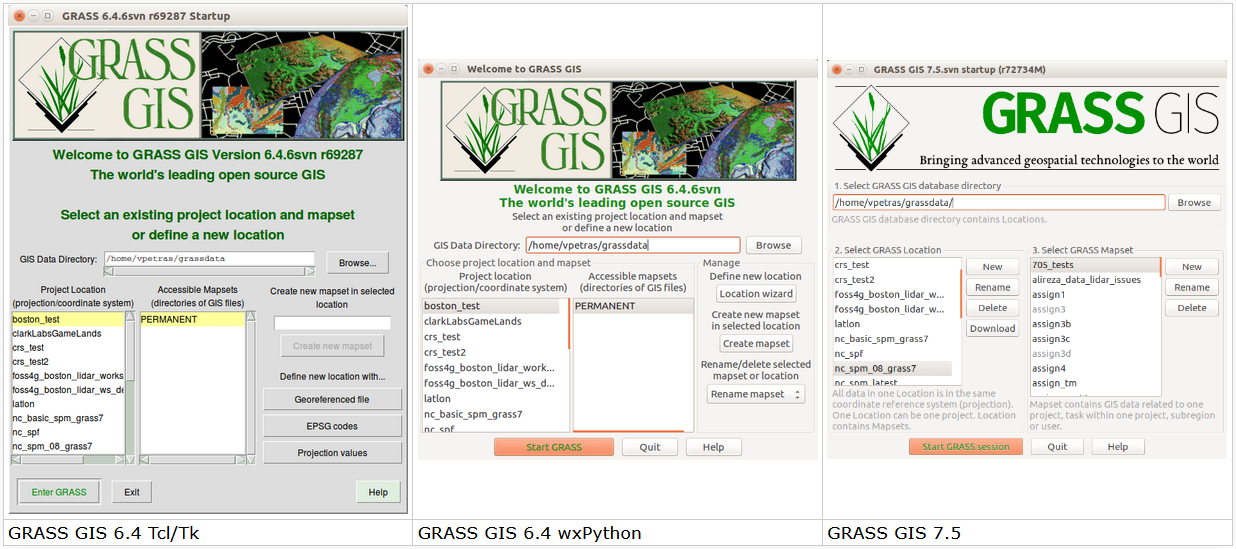
\includegraphics[width=15cm]{pictures/verze_startup.png} 
\caption[Historical versions of the GRASS startup screen]{Historical versions of the GRASS startup screen}
\label{fig:verze_startup}
\end{center}
\end{figure}

Creating a new location and mapset is done using the appropriate "New" button. When creating a new location, the default Location Wizard dialog box opens, which is another important component composed of multiple dialog boxes, whose goal is to create a location with a defined coordinate system. The dialog box in version 7.8 for selecting the coordinate system can be seen in Figure \ref{fig:loc_wizard_sour_pred}.

\vspace{0.3cm}
\begin{figure}[hbt!]
\begin{center}
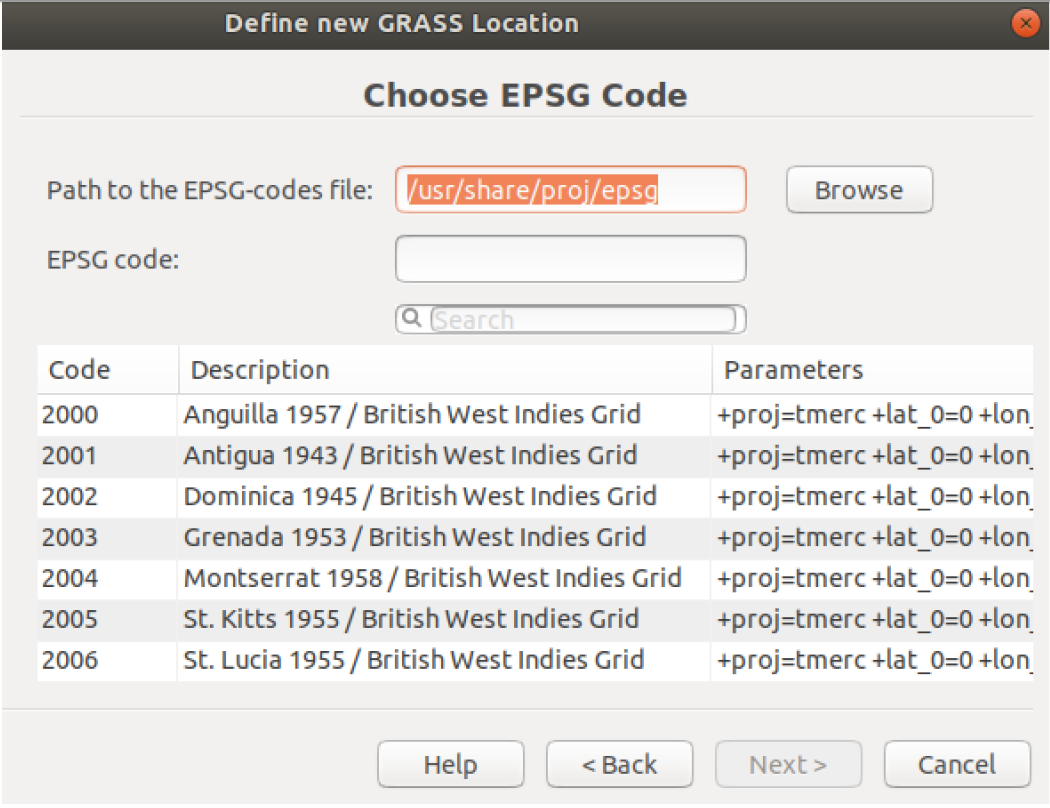
\includegraphics[width=11cm]{pictures/loc_wizard_sour_pred.png} 
\caption[Choosing EPSG code in Location Wizard in version 7.8]{Choosing EPSG code in Location Wizard in version 7.8}
\label{fig:loc_wizard_sour_pred}
\end{center}
\end{figure}

\noindent GRASS GIS is usually run from the command line. Advanced users often do not even run the graphical environment and perform all geographic analyzes using the command line. In our work, however, we mainly focus on first-time users who do not have to be experienced. To summarize, in version 7.8 and earlier, the software can be run from the command line in four ways:

\noindent \textbf{grass78} \\
\noindent Start GRASS using the default user interface. The user will be prompted by the startup screen to choose the appropriate location and mapset.

\noindent \textbf{grass78 --gui}\\
\noindent Start GRASS using the graphical user interface. The user will be prompted by the startup screen to choose the appropriate location and mapset.

\noindent \textbf{grass78 --text} \\
\noindent Start GRASS using the text-based user interface. Appropriate location and mapset must be either set by environmental variables or taken from the last GRASS session.

\noindent \textbf{grass78 --gtext} \\
\noindent Start GRASS using the text-based user interface. The user will be prompted by the startup screen to choose the appropriate location and mapset.

Only the \textbf{grass78 --text} option does not display the startup screen. However, it means that desired location and mapset must already be set as environmental variables, for example by running a specific mapset using the \textbf{grass78 \$HOME/grassdata/location/mapset} command, or taken from the last GRASS session, specifically from a file in the path \textit{\$HOME/.grass7/rc}, which stores the current mapset and current location when the software is closed.

If a GRASS session is launched, the user is redirected to the main software window consisted of two windows - Layer Manager and Map Display. In the Layer Manager first we can see the Layers tab, which allows layers in Map Display to be switched on and off.  After starting the session this tab is empty. The path to the current mapset and location can be noticed in the top bar in the Map Display window as shown in Figure \ref{fig:empty_layers1}. In this case, the current mapset is called \textit{demomapset} and is located in the location named \textit{fire\_grassdata}.

\vspace{0.3cm}
\begin{figure}[hbt!] 
\begin{center}
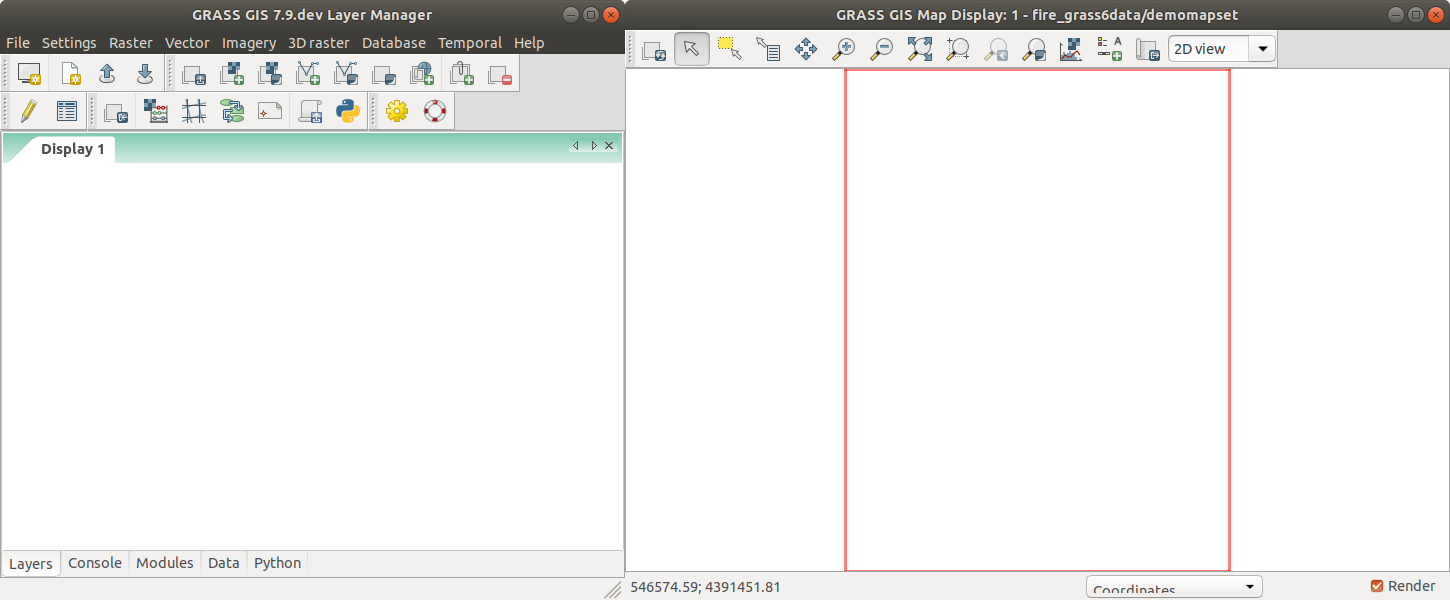
\includegraphics[width=15cm]{pictures/empty_layers1.png} 
\caption[The main software window (version before GSoC)]{The main software window (version before GSoC)}
\label{fig:empty_layers1}
\end{center}
\end{figure}

If we want to display the data located in the current mapset, we need to go to the Data tab. In this tab provided in Figure 
\ref{fig:data_catalog_pred}, there is a Data Catalog (Data Tree) which very nicely captures the hierarchical structure of GRASS components. Within this tree we are allowed to work with layers - to rename, delete, display themselves or their metadata, or to copy layers to another mapset.

\vspace{0.3cm}
\begin{figure}[hbt!] 
\begin{center}
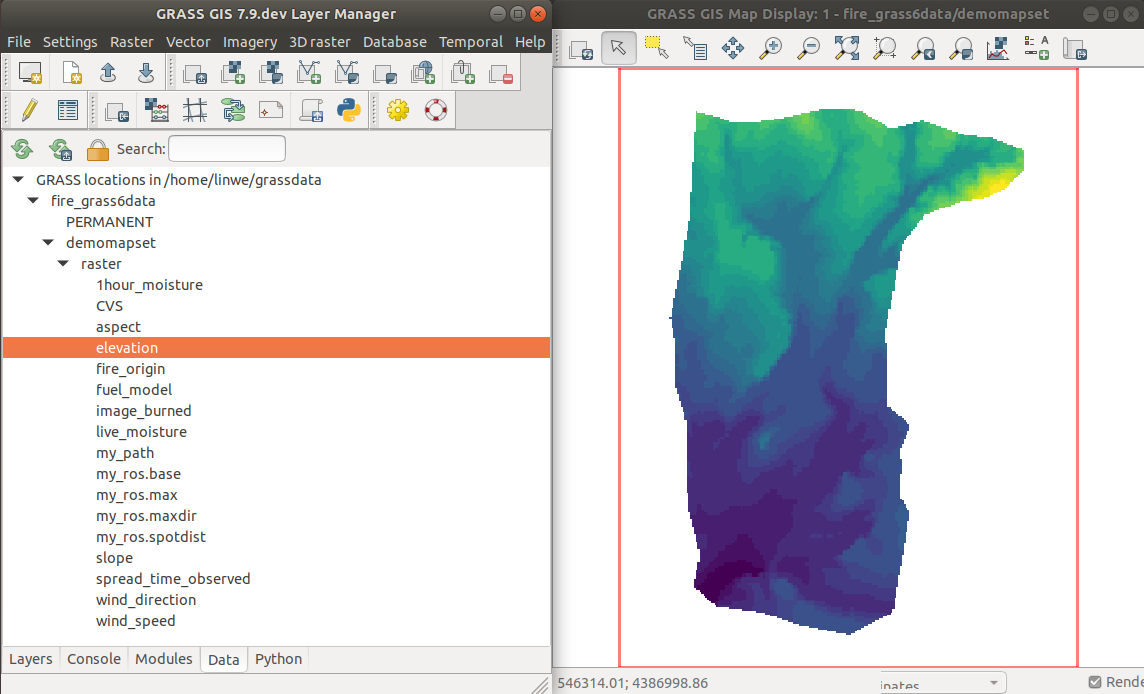
\includegraphics[width=15cm]{pictures/data_catalog_pred.png} 
\caption[Data Catalog in Data tab (version before GSoC)]{Data Catalog in Data tab (version before GSoC)}
\label{fig:data_catalog_pred}
\end{center}
\end{figure}

Since it is always possible to display only map layers from the current mapset, on a mapset node we can find an option for switching. We can switch both - between mapsets in the same location and between mapsets in different locations. Similarly, we can move data. If we move the data to the mapset in another location with a different coordinate system, the projection takes place. We can also notice a lock icon that enables or disables the editing of layers outside the current mapset.

In version 7.8 there are no intuitive functions on the nodes in the Data Catalog that would allow more advanced management of mapsets, locations, or a database. Creating and changing a location or mapset is somewhat hidden in the Settings/GRASS working environment tab.


%% -------<<< Chapter 2: Concepts of startup mechanism >>>-------\\%%%%%%%%%%%%%%%%%%%%%%%%%%%%%%%%%%%%
\newpage
\vspace*{-1cm}
\fancyhead[RE, RO]{\fancyplain{}{\small \sl{General startup concepts}}}
\section{General startup concepts}
\noindent
\large

\noindent Napsat obecně o startovacích mechanismech. Vykročit i mimo GIS, vybrat zástupce různých mechanismů u softwarů a udělat jejich průřez.

\subsection{GIS software}
\subsection{Other software}


%% -------<<< Chapter 3: GRASS GIS startup proposals>>>-------\\%%%%%%%%%%%%%%%%%%%%%%%%%%%%%%%%%%%%
\newpage
\vspace*{-1cm}
\fancyhead[RE, RO]{\fancyplain{}{\small \sl{GRASS GIS startup proposals}}}
\section{GRASS GIS startup proposals}
\noindent
\large

\noindent The mechanism described in the section \ref{State of Art} proved its worth especially when used by experienced users of GRASS, however, for complete beginners, it was rather confusing. The above-mentioned main components (Database, Location, and Mapset) had to be defined right at the start of the software when launching the so-called startup screen. No knowledge of those concepts could discourage many first-time users (I was also among them).

Therefore, the question was whether to keep these components at all or be satisfied only with the Project and with the layers, which is the usual standard for other GIS software. The \texttt{database/location/mapset} mechanism may indeed seem complicated at first glance, but we must keep in mind that many later problems will be avoided by clearly defining the coordinate system at the beginning and allowing only one coordinate system within one Location. For example, it is not possible to display two layers of different coordinate systems on top of each other, as is possible in other GIS software (QGIS, ArcGIS). \textit{\color{red} Opravdu? Změnit na základě kapitoly 2.}

Considering the advantages mentioned above, it seemed very unfortunate to disrupt this system. Rather, it was important to clearly introduce it to first-time users. Over the years, several proposals for changing the current start-up mechanism have been made up.

\subsection{Proposal A1: More newbie-friendly startup}

This design made by Moritz Lennert in Figure \ref{fig:proposalA1} preserves the startup screen but disrupts \texttt{database/location/mapset} system. These components are replaced by components named Project and Mapset. In this sense, the Project has a similar meaning as the Location. However, the startup screen does not operate with a name other than Project since it may be less confusing to first-time users. Only after creating or opening an existing Project, we can see the main software window with the defined Project containing Mapsets. As with the existing solution, the default content of the Project (Location) is PERMANENT Mapset. The user has the option to either create a completely new Project (1st tab), or choose one of the predefined Projects in the second tab (similar to the current Download Location icon), or choose from existing Projects (3rd tab).

\vspace{0.3cm}
\begin{figure}[hbt!] 
\begin{center}
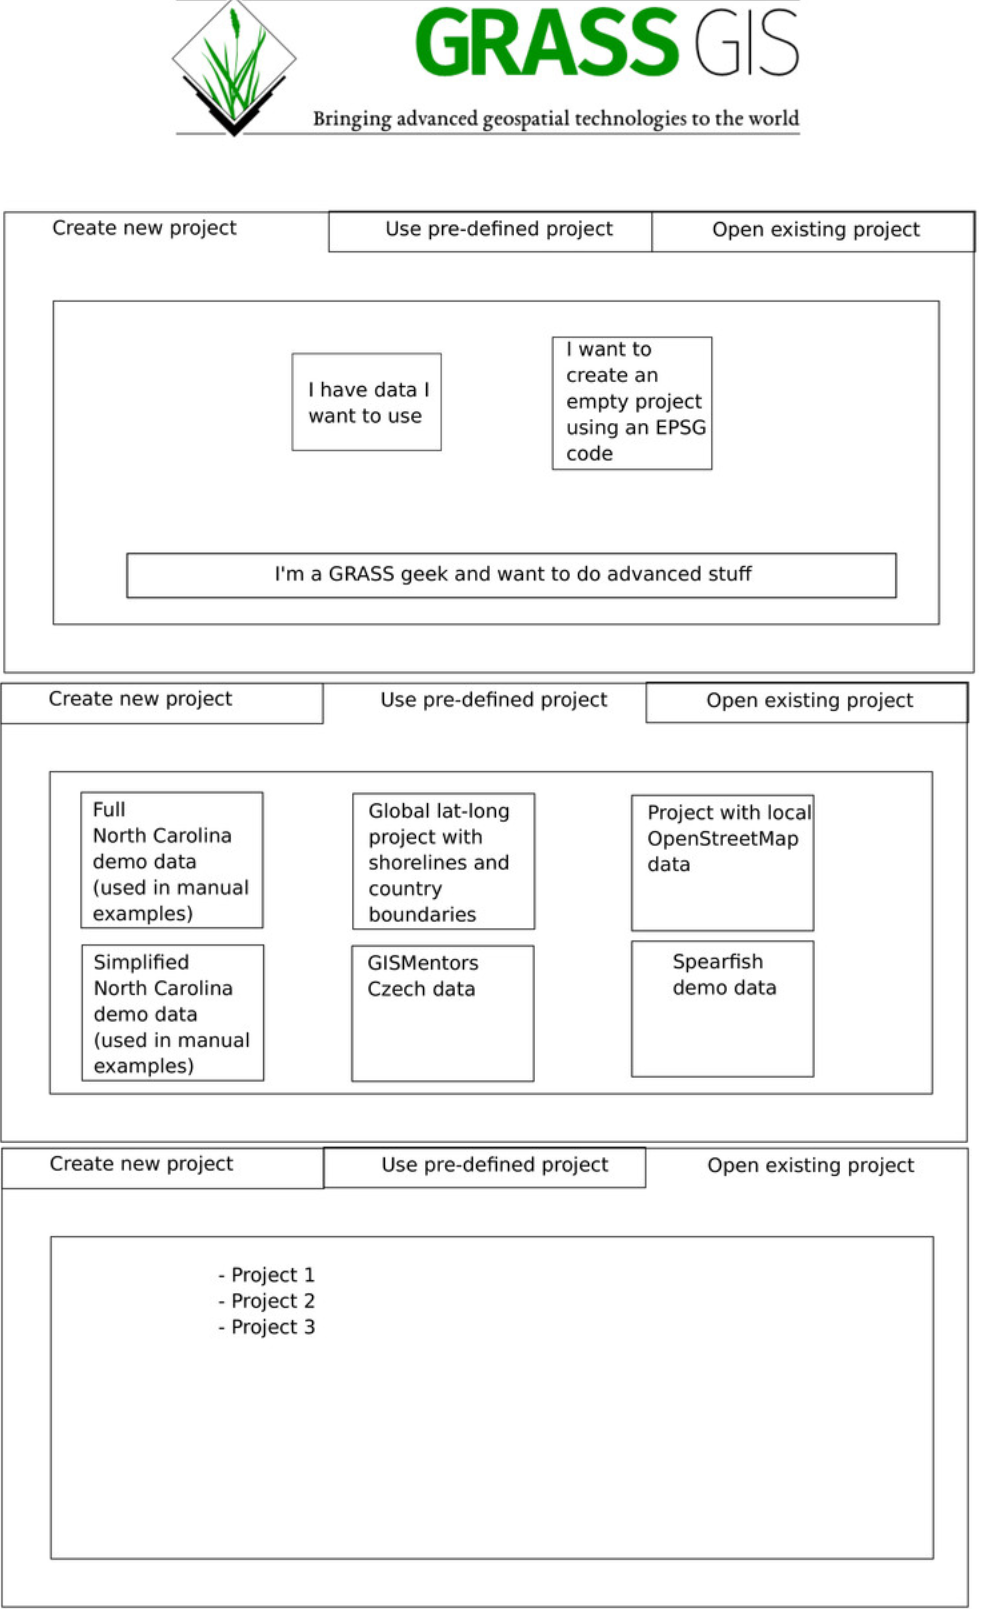
\includegraphics[width=11cm]{pictures/proposalA1.png} 
\caption[Proposal A1 by Moritz Lennert]{Proposal A1 by Moritz Lennert}
\label{fig:proposalA1}
\end{center}
\end{figure}

\textit{\color{red} Porovnat s obecnými startupy jiných softwarů a GIS softwarů, k čemu to má nejblíž?}
\textit{\color{red} Nevýhody?}

\subsection{Proposal B1: Startup as information message}

It is highly important to mention this suggestion here, because it somewhat changes the perspective of how we can perceive the startup mechanism.  Again, the \texttt{database/location/mapset} mechanism is replaced by the \texttt{project/mapset} paradigm. Moritz Lennert followed up on the proposal A1 design and subsequently simplified it.

As soon as GRASS started, the main software window containing the Layer Manager and Map Display together with pre-prepared map is shown up (Figure \ref{fig:proposalB1}). By default, the lat-long coordinate system is set. Before the user can interact, a message is displayed informing him about the importance of the projection option for spatial analysis. The user can opt to get out of this report and simply explore GRASS GIS in the default Location or create a new Project with his own data. This proposal seems quite intuitive. Although it displays the startup screen, its sense is now rather informative.

\vspace{0.3cm}
\begin{figure}[hbt!] 
\begin{center}
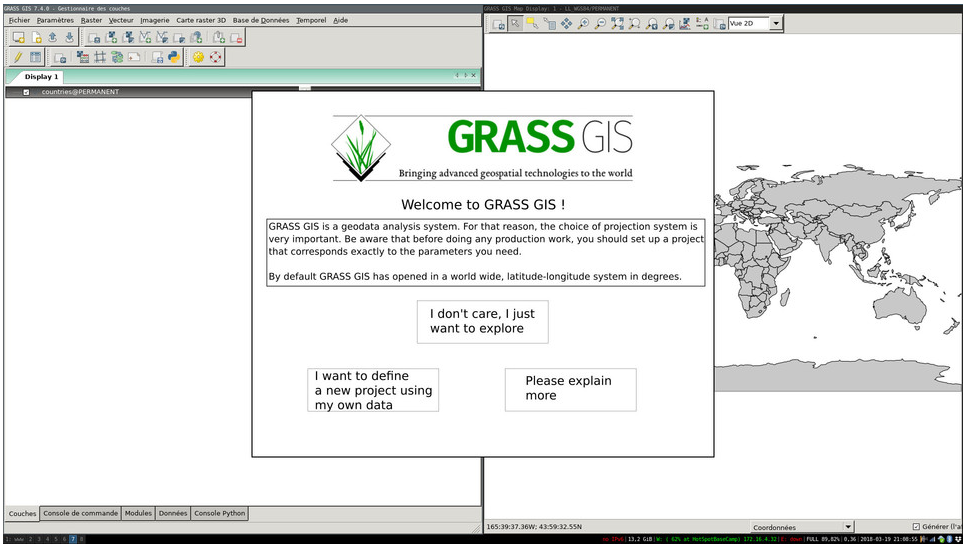
\includegraphics[width=15cm]{pictures/proposalB1.png} 
\caption[Proposal B1 by Moritz Lennert]{Proposal B1 by Moritz Lennert}
\label{fig:proposalB1}
\end{center}
\end{figure}

\textit{\color{red} Porovnat s obecnými startupy jiných softwarů a GIS softwarů, k čemu to má nejblíž?}
\textit{\color{red} Nevýhody?}

\subsection{Proposal A2: Well-designed tabs on the side}

This proposal written by Garrett Millar tries to make the start screen clearer and also add more functionality within it. It is based on quick access via well-designed tabs on the "New", "Recent" and "Open" tabs. When users first open GRASS, a splash screen appears instead of simply opening one of the three tabs. It happens because users do not become frustrated when seeing options they do not need. 

The design changes the \texttt{database/location/mapset} paradigm a bit. On the "New" tab, we can still define a new location by opening an existing Location Wizard dialog box or defining a location from a template as especially first-time users just want to explore. After the Location definition, we can use existing data to create a new Mapset or new Workspace. Workspace is a new concept here, and to create it, a user must select an existing Location and Mapset for which a new Workspace is created.

In the "Recent" tab, a user can choose from recently used Locations, Mapsets, or Workspaces. The third tab called "Open" allows to open existing GRASS data. At the top, we can see the current Database directory, which can be changed. At the same time, the "Open existing GRASS data" window displays the data in the Database in the same Data Catalog (Data Tree) structure as the "Data" tab in the Layer Manager. It captures the bottom right corner of Figure \ref{fig:proposalA2}. Only Databases, Locations, and Mapsets are shown in the "Open existing GRASS data" window, a Workspace may be shown as well. We can notice that unlike Figure \ref{fig:empty_layers1} each data type is displayed with a corresponding icon for easy identification. The "Selected data" is displayed again on the right (same function as on the "Recent" tab).

\vspace{0.3cm}
\begin{figure}[hbt!] 
\begin{center}
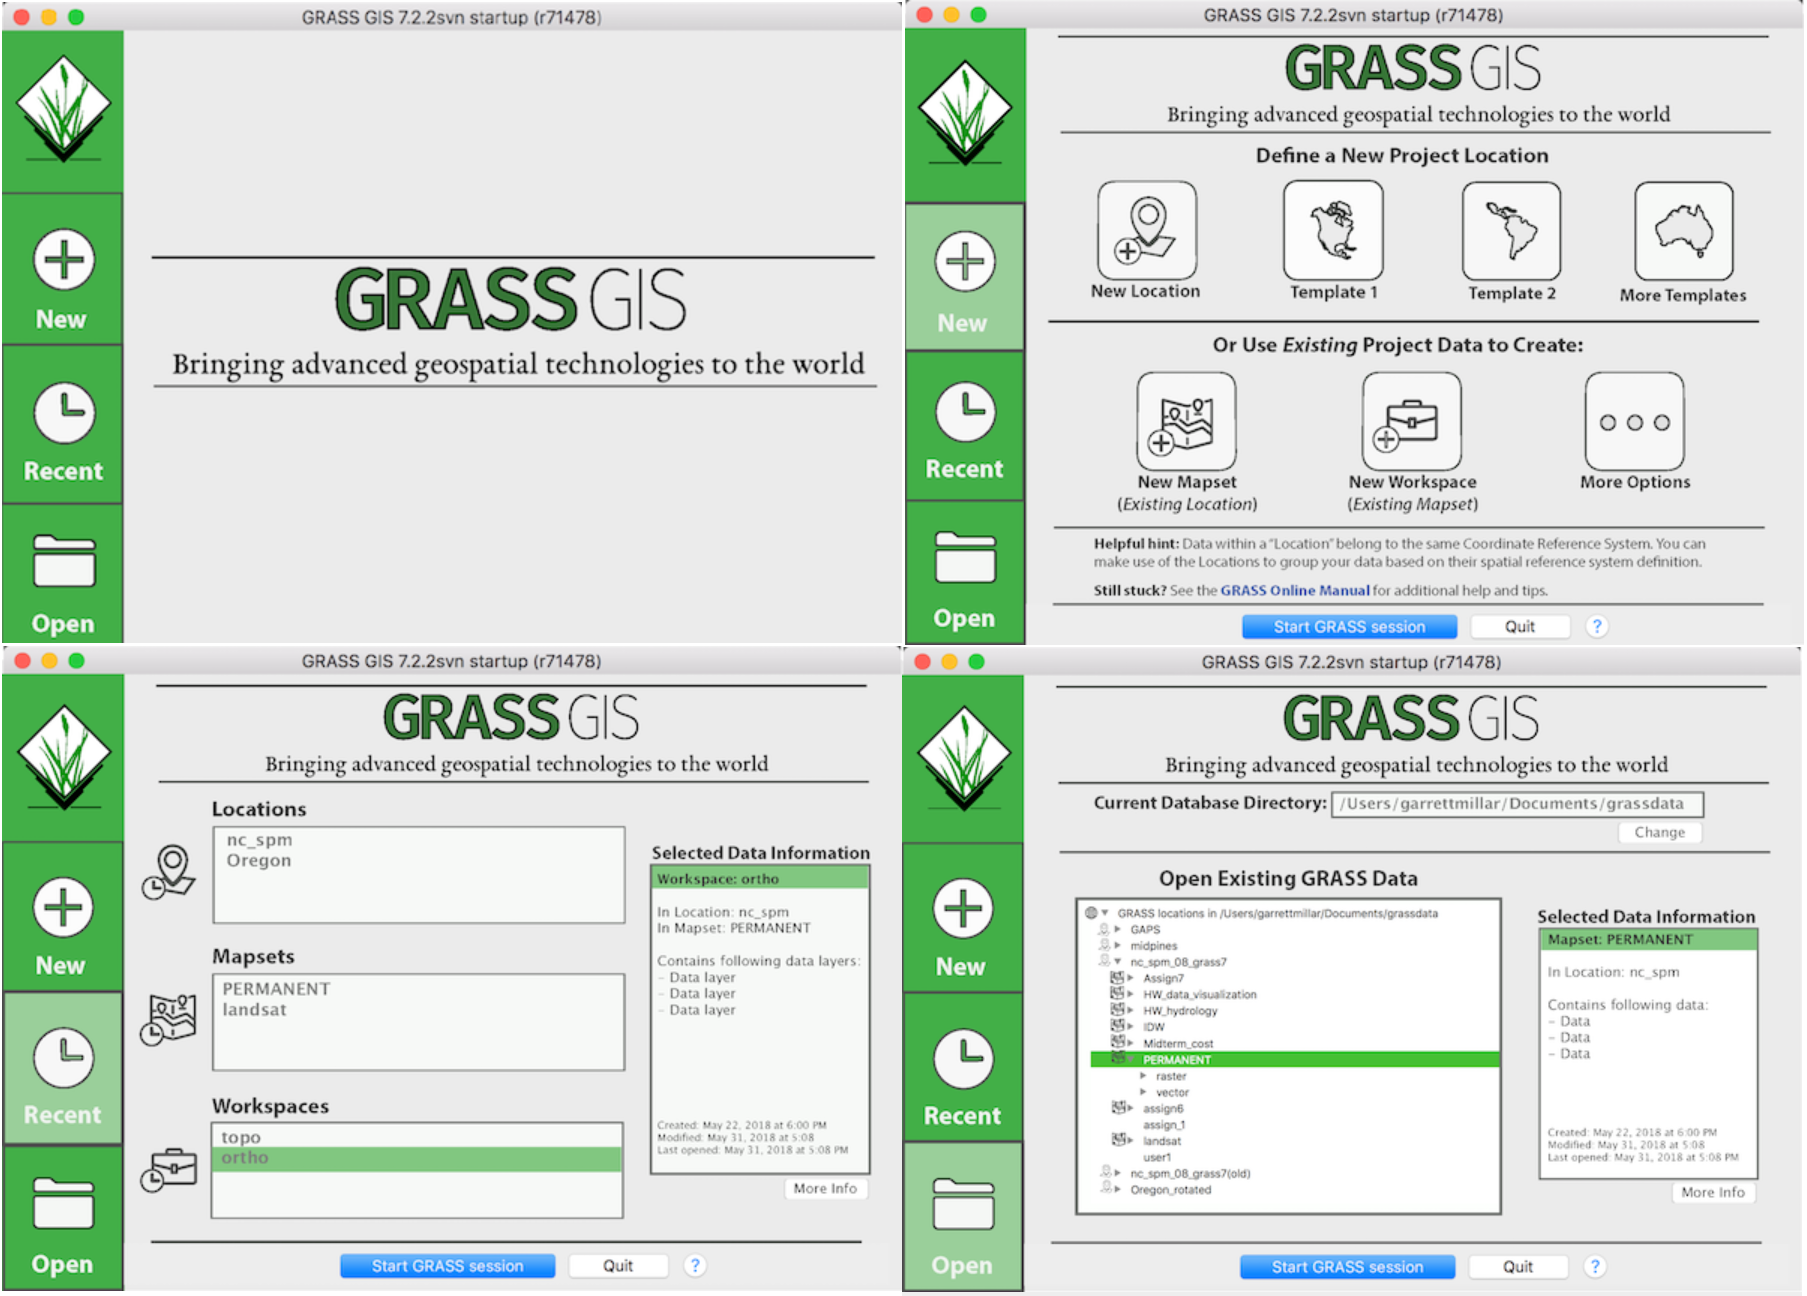
\includegraphics[width=15cm]{pictures/proposalA2.png} 
\caption[Proposal A2 by Garrett Millar]{Proposal A2 by Garrett Millar}
\label{fig:proposalA2}
\end{center}
\end{figure}

\textit{\color{red} Porovnat s obecnými startupy jiných softwarů a GIS softwarů, k čemu to má nejblíž?}
\textit{\color{red} Nevýhody?}

\subsection{Proposal A3: Data tree and big buttons}

This proposal was discussed in more detail in Prague in 2019 and an implementation process was created, available as the Prague Roadmap at \url{https://trac.osgeo.org/grass/wiki/wxGUIDevelopment/New\_Startup\#PragueRoadmap}.

The database/location/mapset concept is preserved again. The main points of this suggestion were the improvement of the existing Location Wizard guide and the Data Catalog located in the Data tab. In this proposal, it is necessary to take into account a new concept called Workspaces, which is not directly part of the Mapset, but is associated with it. The proposed changes in the Location Wizard are mainly related to the clarification of the first page, better naming of the given attributes and speeding up the selection of the coordinate system in the dialog, whose original version was introduced in Figure \ref{fig:loc_wizard_sour_pred}.

The most serious changes concern the Data Catalog. They lies in supporting multiple databases, adding buttons to create existing or new databases, or adding new actions from the context menu to a database, location, and mapset node. The same Data Catalog implemented in the Data tab will then be used within Startup screen which is inspired by A2 proposal designed by Garrett Millar. However, unlike the A2 design, the Startup screen has no other tabs. It consists of only one startup page, which has a Data Datalog (Data Tree) in the center, and a toolbar with big buttons for creating or defining new or existing components, such as a Location or Mapset. 

The proposal assumes the possibility of filtering in the Data Catalog based on the recently selected items. General startup GUI should to be able to collect recent maps and workspaces as well as used databases and workspaces. The display of map layers in the Data Catalog is switched off by default, the display of workspaces under the relevant mapset is switched on. When GRASS GIS launches, a "grassdata" directory should be automatically created in a reasonable place, which is the meaning of the database in which locations, maps and map layers are stored.

\textit{\color{red} Porovnat s obecnými startupy jiných softwarů a GIS softwarů, k čemu to má nejblíž?}
\textit{\color{red} Nevýhody?}


%% -------<<< Chapter 4: Used technologies>>>-------\\%%%%%%%%%%%%%%%%%%%%%%%%%%%%%%%%%%%%
\newpage
\vspace*{-1cm}
\fancyhead[RE, RO]{\fancyplain{}{\small \sl{Used technologies}}}
\section{Used technologies}
\noindent
\large

\noindent This chapter briefly presents GRASS GIS, a Geographic Information System (GIS) technology built for vector and raster geospatial data management, geoprocessing, spatial modelling and visualization, from both historical and technical point of view. Furthermore, it describes the main programming technology used for a new startup GUI implementation, called wxPython.

\subsection{GRASS GIS}
\noindent
\large

\noindent GRASS (Geographic Resources Analysis Support System) is a cross-platform desktop geographic information system (GIS) designed to work with geographic 2D/3D raster and vector data, image records, both using the command line and graphical user interface (GUI). Besides, it enables the production of high-quality graphic outputs, spatio-temporal modeling, data visualization, or connection to spatial databases.

The development of the GRASS GIS system was started by the research laboratories of the US Army Engineer Engineer in 1982, later got into the academic sphere and today it is also used in the commercial sphere. It is open-source software published under the GNU GPL general license and managed and developed under the OSGeo organization. Important users of the GRASS system include, for example, NASA or NOAA.

The power of software stems mainly from its Unix philosophy, where the software itself consists of a collection of more than 500 applications called modules. Each of these modules has only one task to perform, and the real power of the software comes when the various of these modules begin to chain together, allowing the user to create even very complex applications. Most of these modules are written in C, but above the whole system, PyGRASS as an object-oriented Python Application Programming Interface (API) stands, which hides the complexity of GRASS and provides access to the capability of the C- API of GRASS for geo-scientists that are not familiar with C.

Nowadays, most main changes take place in the python programming language, which also applies to the GUI, which uses the wxPython extension. The software has been developing since January 2020 on GitHub, a web service that supports development using the Git versioning tool. This principle makes working on code much clearer. It stores the history of work, ensures stylistic consistency using the flake8 command-line utility, and also allows the creation of Issues, which can have the character of errors and various improvements. Then these issues are usually proposed for changes (so-called pull requests), which users discuss. Therefore, GitHub partly works as a social network, which can support the creativity and enthusiasm of developers.

At this point, I would like to mention that besides improving the GRASS GIS startup mechanism, in summer 2020 the community presented a new website on the occasion of its 37th birthday (stable version 7.8.) which offers a curated list of tutorials in different languages and links to videos.

\vspace{0.3cm}
\begin{figure}[hbt!]
\begin{center}

\includegraphics[width=15cm]{pictures/grass_gis.png} 
\caption[New GRASS website's layout]{New GRASS website's layout (source: \url{https://grass.osgeo.org)}}
\label{fig:grass_gis}
\end{center}
\end{figure}

\subsection{wxPython}
\noindent
\large

\noindent This open-source toolkit allows Python programmers to create a graphical user interface. We can import it to a script file as a package that wraps the GUI components of the popular wxWidgets cross-platform C++ library established in 1992 at the Artificial Intelligence Applications Institute at University of Edinburgh. There are a number of other graphical user interface (GUI) packages for Python, for example, the Tkinter package is also very popular.

wxPython is a cross-platform toolkit which means that the same program can be run on multiple platforms without modification. Currently, supported platforms are Windows, macOS, Linux, or other Unix-like systems. The resulting design on each platform can be a bit different as we can also notice when using GRASS GIS on different systems. 


%% -------<<< Chapter 3: Implementation>>>-------\\%%%%%%%%%%%%%%%%%%%%%%%%%%%%%%%%%%%%
\newpage
\vspace*{-1cm}
\fancyhead[RE, RO]{\fancyplain{}{\small \sl{Implementation}}}
\section{Implementation}
\noindent
\large

%% -------<<< Chapter: Discussion >>>-------\\%%%%%%%%%%%%%%%%%%%%%%%%%%%%%%%%%%%%
\newpage
\vspace*{-1cm}
\fancyhead[RE, RO]{\fancyplain{}{\small \sl{Discussion}}}
\section*{Discussion}
\addcontentsline{toc}{section}{Discussion}
\noindent
\large

%% -------<<< Chapter: Conclusion >>>-------\\%%%%%%%%%%%%%%%%%%%%%%%%%%%%%%%%%%%%
\newpage
\vspace*{-1cm}
\fancyhead[RE, RO]{\fancyplain{}{\small \sl{Conclusion}}}
\section*{Conclusion}
\addcontentsline{toc}{section}{Conclusion}
\noindent
\large

%% -------<<< Chapter: List of abbreviations >>>-------\\%%%%%%%%%%%%%%%%%%%%%%%%%%%%%%%%%%%%
\newpage
\vspace*{-1cm}
\fancyhead[RE, RO]{\fancyplain{}{\small \sl{List of abbreviations}}}
\section*{List of abbreviations}
\addcontentsline{toc}{section}{List of abbreviations}
\noindent
\large


%% -------<<< LITERATURA >>>-------\\%%%%%%%%%%%%%%%%%%%%%%%%%%%%%%%%%%%%%%%
\newpage
\vspace*{-6ex}
\renewcommand{\refname}{Bibliography} 
\addcontentsline{toc}{section}{Bibliography}
\fancyhead[RE, RO]{\fancyplain{}{\small \sl{Bibliography}}}
	\selectlanguage{english}
	\bibliographystyle{plain}
	\bibliography{bibliography}

\noindent
\large

https://trac.osgeo.org/grass/wiki/wxGUIDevelopment/New\_Startup\#PragueRoadmap \\

Zambelli, P.; Gebbert, S.; Ciolli, M. Pygrass: An Object Oriented Python Application Programming Interface (API) for Geographic Resources Analysis Support System (GRASS) Geographic Information System (GIS). ISPRS Int. J. Geo-Inf. 2013, 2, 201-219. \\

Predicting Database Requirements for Geographic Information Systems in the Year 2000: Long-Term Design Issues for GRASS. August 1992.\\

Goran, W.D., Dvorak, W.E., Van Warren, L. and Webster, R.D., 1983, Fort Hood Geographic Information System: Pilot System Development and User Instructions, Technical Report N-154, USA Construction Engineering Research Laboratory, Champaign, IL.\\

https://www.wxpython.org/\\

https://grass.osgeo.org/\\


\end{document}
